\documentclass[tikz,border=8pt]{standalone}
% Shared look for every TikZ diagram. Load with \input{../../tools/tikz-style.tex}
\usepackage[T1]{fontenc}
\usepackage{lmodern}
\renewcommand{\sfdefault}{lmr}  % diagrams use the same serif as the text
\usetikzlibrary{arrows.meta, positioning, shapes.geometric, calc, fit, backgrounds}
\definecolor{cblue}{HTML}{4C78A8}
\definecolor{corange}{HTML}{F58518}
\definecolor{cgreen}{HTML}{54A24B}
\definecolor{cred}{HTML}{E45756}
\definecolor{cpurple}{HTML}{B279A2}
\definecolor{cgrey}{HTML}{6B6B6B}
\tikzset{
  every picture/.style={font=\sffamily, line width=1.2pt},
  box/.style={draw=#1, fill=#1!12, rounded corners=4pt, align=center, inner sep=7pt, minimum height=1.1cm},
  box/.default=cgrey,
  arrow/.style={-{Stealth[length=3mm]}, draw=cgrey, line width=1.4pt},
  title/.style={font=\sffamily\bfseries\Large},
  note/.style={font=\sffamily\small, text=cgrey, align=center},
}
\AtBeginDocument{\hyphenpenalty=10000 \exhyphenpenalty=10000}

\begin{document}
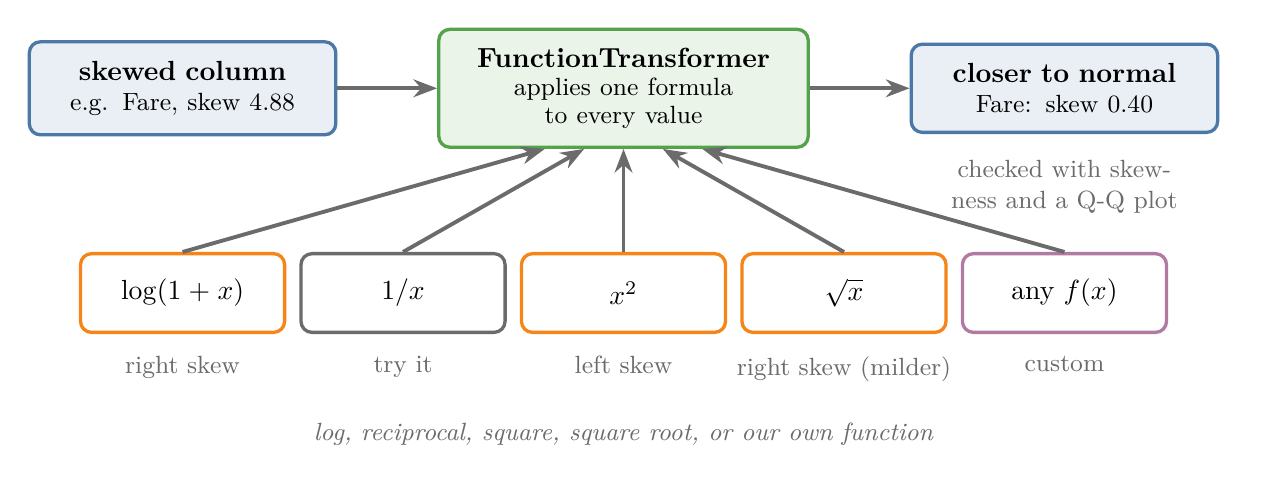
\begin{tikzpicture}
  \node[box=cblue, text width=3.4cm] (in) at (0,0) {\textbf{skewed column}\\[-1pt]\small e.g. Fare, skew 4.88};
  \node[box=cgreen, text width=4.2cm, minimum height=1.4cm] (ft) at (5.6,0)
    {\textbf{FunctionTransformer}\\[-1pt]\small applies one formula\\[-2pt]\small to every value};
  \node[box=cblue, text width=3.4cm] (out) at (11.2,0) {\textbf{closer to normal}\\[-1pt]\small Fare: skew 0.40};
  \draw[arrow] (in) -- (ft);
  \draw[arrow] (ft) -- (out);
  \foreach \i/\f/\w/\c in {0/{$\log(1+x)$}/right skew/corange, 1/{$1/x$}/try it/cgrey,
                           2/{$x^2$}/left skew/corange, 3/{$\sqrt{x}$}/right skew (milder)/corange,
                           4/{any $f(x)$}/custom/cpurple} {
    \node[box=\c, fill=white, text width=2.1cm, minimum height=1cm] (f\i) at ({5.6+2.8*(\i-2)},-2.6) {\f};
    \node[note, below=0.15cm of f\i] {\w};
    \draw[arrow] (f\i.north) -- ($(ft.south)+({0.5*(\i-2)},0)$);
  }
  \node[note, font=\sffamily\small\itshape] at (5.6,-4.4) {log, reciprocal, square, square root, or our own function};
  \node[note, text width=4.5cm] at (11.2,-1.25) {checked with skewness and a Q-Q plot};
\end{tikzpicture}
\end{document}
